\documentclass[10pt,a4paper]{article}
\usepackage[utf8]{inputenc}
\usepackage{amsmath}
\usepackage{amsfonts}
\usepackage{amssymb}
\usepackage{graphicx}
\usepackage{ulem}
\author{Ferdous Nasri \\ Yannek Nowatzky \\ Leli Schiestl}
\title{Datenbanksysteme Projekt}
\begin{document}
	\maketitle
	\newpage
	\section{Projektiteration}
	\subsection{ERM anhand der Projektbeschreibung und Daten erstellen}
	Zuerst haben wir anhand der Anforderungen ein ERM erstellt. Beim späteren Abgleichen mit der Datenbank ist uns aufgefallen, dass wir nicht alle Informationen aus der Datenbank herauslesen können, die wir laut Beschreibung benötigen.\\ \\	
	\begin{figure}[h]
		\centering
		\includegraphics[width=1\linewidth]{ERMalt}
		\caption[ERM der ersten Projektiteration]{ERM der ersten Projektiteration der Datenbank greyhounddog}
		\label{fig:ERMalt}
	\end{figure}
	
	\subsection{Relationales Modell ableiten }
	Aus dem ERM (Figure \ref{fig:ERMalt}) leiten wir nun das Relationale Modell ab.\\
	\\\textsf{
	\textbf{Dog(\underline{name}, year\_of\_birth, land\_of\_birth, land\_of\_standing, sex, \uwave{mother}, \uwave{father}, \uwave{owner}, \uwave{breeder})
	\\ \\
	Race(\underline{country, year})
	\\ \\
	participated\_in(\uwave{\uline{dog\_name, race\_country, race\_year}}, score, average distance, rank, number\_of\_races)}}
	\\ \\
	Die unterstrichenen Einträge stellen die \texttt{primary keys} dar und die unterwellten Einträge sind \texttt{foreign keys}.
	\subsection{CREATE-Statements zur Erzeugung der Tabellen schreiben}
		Aus diesem rationalen Modell haben wir dann die CREATE Statements abgeleitet.
		\\ \\
		\texttt{	
			CREATE TABLE Dog(\\
				\hspace*{4mm}	name varchar(255) NOT NULL,\\
				\hspace*{4mm}	year\_of\_birth int,\\
				\hspace*{4mm}	land\_of\_birth nchar(2),\\
				\hspace*{4mm}	land\_of\_standing nchar(2),\\
				\hspace*{4mm}	sex nchar(1),\\
				\hspace*{4mm}	father varchar(255),\\
				\hspace*{4mm}	mother varchar(255),\\
				\hspace*{4mm}	owner varchar(255),\\
				\hspace*{4mm}	breeder varchar(255),\\
				\hspace*{4mm}	CONSTRAINT pk\_dog PRIMARY KEY (name),\\
				\hspace*{4mm}	CONSTRAINT fk\_mother FOREIGN KEY (mother) REFERENCE Dog(name),\\
				\hspace*{4mm}	CONSTRAINT fk\_father FOREIGN KEY (father) REFERENCE Dog(name)\\
			);\\ \\
			CREATE TABLE Race(\\
				\hspace*{4mm}	country varchar(255),\\
				\hspace*{4mm}	year int,\\
				\hspace*{4mm}	CONSTRAINT pk\_race PRIMARY KEY (country, year),\\
			);\\ \\
			CREATE TABLE participated\_in(\\
				\hspace*{4mm}	dog\_name varchar(255),\\
				\hspace*{4mm}	race\_country varchar(255),\\
				\hspace*{4mm}	race\_year int,\\
				\hspace*{4mm}	score float,\\
				\hspace*{4mm}	average\_distance float,\\
				\hspace*{4mm}	CONSTRAINT fk\_dog\_name FOREIGN KEY (dog\_name) REFERENCES Dog(name),\\
				\hspace*{4mm}	CONSTRAINT fk\_race\_country FOREIGN KEY (race\_country, race\_year) \\
				\hspace*{4mm}	REFERENCE Race(country, year)	\\
		);\\}\\ \\
		Bei der Präsentation hat unser Tutor Alexander Korzec uns in der Annahme bestätigt, dass es unmöglich ist aus der Datenbank den Besitzer zu ermitteln und nicht wirklich möglich ist den Züchter zu ermitteln. Daher haben wir für die nächsten Projektiterationen unser Modell angepasst und diese Informationen entfernt.
		\newpage
\section{Projektiteration}
	Für den zweiten Teil der Projektphase haben wir unser ERM angepasst.
	\begin{figure}[h]
		\centering
		\includegraphics[width=0.4\linewidth]{ERMneu}
		\caption{ERM der zweiten Projektiteration den Datenbank greyhounddog}
		\label{fig:ERMneu}
	\end{figure} 
	\\
	Zum einen haben wir den Züchter und den Besitzer entfernt, da wir diese Daten nicht wirklich erfassen konnten. Zum anderen haben wir die Attribute \texttt{land\_of\_standing} und \texttt{land\_of\_birth} zu einem gemeinsamen Attribut zusammengefasst. Dies liegt daran, dass nicht alle Hunde zwei Einträge haben und wir nicht genau wissen, zu welchem der beiden Attribute die einzelnen Einträge gehören.\\ 
	\\
	Dadurch hat sich natürlich auch unser relationales Modell verändert.\\
	\\
	\\\textsf{
		\textbf{Dog(\underline{name}, year\_of\_birth, land\_of\_birth\_and\_standing, sex, mother, father)
		\\ \\
		Race(\underline{country, year})
		\\ \\
		participated\_in(\uwave{\uline{dog\_name, race\_country, race\_year}}, score, average distance,  rank, number\_of\_races )}}
	\\ \\ \\
	Beim einfügen der Daten in die Datenbank haben uns auch dagegen entschieden \texttt{mother} und \texttt{father} als \texttt{foreign keys} beizubehalten, da sonst alle Einträge für Eltern, die nicht selbst Rennhunde in der Datenbank sind \texttt{NULL} gesetzt werden würden. Dadurch gewinnt man nicht wirklich wichtige Informationen und löscht Informationen, die man hat.
	\subsection{Import der Daten über SQL}
	\texttt{CREATE TABLE Dog(\\
		\hspace*{4mm}	name varchar(255) NOT NULL,	\\
		\hspace*{4mm}	year\_of\_birth int,	\\
		\hspace*{4mm}	land\_of\_birth\_and\_standing nchar(5),	\\
		\hspace*{4mm}	sex nchar(1),	\\
		\hspace*{4mm}	father varchar(255),\\
		\hspace*{4mm}	mother varchar(255),\\
		\hspace*{4mm}	CONSTRAINT pk\_dog PRIMARY KEY (name)\\
		);\\
		\\
		CREATE TABLE Race(\\
		\hspace*{4mm}	country varchar(255),\\
		\hspace*{4mm}	year int,\\
		\hspace*{4mm}	CONSTRAINT pk\_race PRIMARY KEY (country, year)\\
		);\\
		\\
		CREATE TABLE participated\_in(\\
		\hspace*{4mm}	dog\_name VARCHAR(255),\\
		\hspace*{4mm}	race\_country VARCHAR(255),\\
		\hspace*{4mm}	race\_year INT,\\
		\hspace*{4mm}	score FLOAT,\\
		\hspace*{4mm}	average\_distance INT,\\
		\hspace*{4mm}	rank INT,\\
		\hspace*{4mm}	number\_of\_races INT,\\
		\hspace*{4mm}	CONSTRAINT fk\_dog\_name FOREIGN KEY (dog\_name) REFERENCES Dog(name),\\
		\hspace*{4mm}	CONSTRAINT fk\_race FOREIGN KEY (race\_country, race\_year) REFERENCES \\ \hspace*{4mm}	Race(country, year)\\
		); }
	\\ \\
	Außerdem haben wir eine Hilfstabelle für den Import der Daten aus der Datei greyhounddata.csv erstellt.
	\\ \\
	\texttt{
		CREATE TABLE import(\\
		\hspace*{4mm}	i\_country VARCHAR(255),\\
		\hspace*{4mm}	i\_year int,\\
		\hspace*{4mm}	i\_rang int,\\
		\hspace*{4mm}	i\_name VARCHAR(255),\\
		\hspace*{4mm}	i\_sex CHAR,\\
		\hspace*{4mm}	i\_vater VARCHAR(255),\\
		\hspace*{4mm}	i\_mutter VARCHAR(255),\\
		\hspace*{4mm}	i\_anzahl int,\\
		\hspace*{4mm}	i\_punkte DOUBLE PRECISION,\\
		\hspace*{4mm}	i\_durch VARCHAR(30)\\
		);\\
		}
	\newpage
	\noindent In diese \texttt{import} importieren wir die Daten mit folgendem Befehl:\\ \\
	\texttt{
		COPY import(i\_country, i\_year, i\_rang, i\_name, i\_sex, i\_vater, i\_mutter, i\_anzahl, i\_punkte, i\_durch)\\
		FROM '/Users/Shared/greyhounddata.csv'\\
		WITH DELIMITER ';';\\
		}
 	\subsection{Bereinigung der Daten}
 Da die Daten nicht alle in dem von uns gewünschten Format vorlagen, haben wir eine zweite Hilfstabelle import2 angelegt. \\ \\
 \\
 \texttt{
 	CREATE TABLE import2(\\
 	\hspace*{4mm}	i2\_country VARCHAR(255),\\
 	\hspace*{4mm}	i2\_year INT,\\
 	\hspace*{4mm}	i2\_rang INT,\\
 	\hspace*{4mm}	i2\_name VARCHAR(255),\\
 	\hspace*{4mm}	i2\_year\_of\_birth VARCHAR(255),\\
 	\hspace*{4mm}	i2\_land\_of\_birth\_and\_standing VARCHAR(255),\\
 	\hspace*{4mm}	i2\_sex CHAR,\\
 	\hspace*{4mm}	i2\_vater VARCHAR(255),\\
 	\hspace*{4mm}	i2\_mutter VARCHAR(255),\\
 	\hspace*{4mm}	i2\_anzahl INT,\\
 	\hspace*{4mm}	i2\_punkte FLOAT,\\
 	\hspace*{4mm}	i2\_durch VARCHAR(30)\\
 	);\\
 	\\}
  \\
  Der Lesbarkeit zu Liebe fügen wir hier nicht alle Import Befehle für die Tabelle \texttt{import2} ein und verweisen auf die Quellcode-Datein.\\ \\
  Die Spalten für \texttt{country}, \texttt{year}, \texttt{rang, sex, vater, mutter} und \texttt{anzahl der rennen} wurden einfach kopiert. \\
  Da der Name in der Ursprungsdatei aus dem Namen, dem Geburtsjahr, dem Geburtsland und dem Rennland bestand, haben wir diese Information mithilfe von \texttt{substring} in die jeweiligen Spalten \texttt{i2\_name}, \texttt{i2\_year\_of\_birth}, \\ \texttt{i2\_land\_of\_birth\_and\_standing } von \texttt{import2} kopiert.\\ \\
  Als Beispiel führen wir hier die Gewinnung des Namens an:\\ \\
  \texttt{substring(i\_name for position('[' in i\_name)-2)} \\ \\
  Die Punkte sollten wir runden, daher haben wir beim kopieren in \texttt{import2} den Befehl \texttt{round(i\_punkte)} angewandt.\\
  Da die durchschnittliche Renndistanz mit dem Zusatz 'm' zu einem String wurde, haben wir auch hier den \texttt{substring} gebildet und alles was keine Zahl war, abgeschnitten.\\ 
  \\
  Dann haben wir die Werte in die drei Tabellen \texttt{Dog}, \texttt{Race} und \texttt{participated\_in} eingefügt. Dabei haben wir die beiden Strings \texttt{year\_of\_birth} und \texttt{average\_distance} mit dem Befehl \texttt{::INTEGER} in Integer umgewandelt. Um redundante Tabelleneinträge zu vermeiden, haben wir \texttt{DISTINCT} eingefügt.\\  
  \\
  Als Beispiel führen wir hier die Tabelle \texttt{Race} an.\\ \\
  \texttt{  INSERT INTO Race(country, year)\\
  \hspace*{2mm}	SELECT DISTINCT i2\_country, i2\_year FROM import2;}
\subsection{API (vorerst für Konsolenanwendungen)}
API wird unter 3.2 im Rahmen der Web-GUI erläutert. In dieser Iteration wurde noch auf die GUI-Umsetzung verzichtet, die SQL-Code Eingabe erfolgt über Konsole und konnte so direkt in Java behandelt werden.
	\newpage
	\section{Projektiteration}
	\subsection{Entwurf und Umsetzung einer Web-GUI (HTML/CSS)}
	Um unsere Resultaten schön darzustellen und die Query benutzerfreundlicher ausführen zu können, haben wir ein Web-GUI gebaut. Da hatten wir viel Designentscheidungen zu treffen. Wir haben uns entschieden ausschliesslich die Sprachen HTML und CSS zu benutzen (Die schon geschriebene Code auf sass, scss und ReactJS worden dann zu einfache CSS übersetzt.). Erstens haben wir unsere Dog-Query Seite erstellt und dabei gemerkt dass wir ein "Willkommen Seite" brauchen wo Users sich entschieden können, ob sie die Daten von einer spezifischer Hund sehen möchten oder ob sie die Vorhersagen von Hunden sehen möchten.
Dabei haben wir die Navigationsbar auch hergestellt. Ganz zum Schluss sahen die Seiten einigermassen in Ordnung aus (nach der Behebung von viel kleine Designfehler). Anbei paar Screenschots von unsere Webseite. 
	\subsection{Java API – Schnittstelle zwischen Datenbankzugriff (SQL) und GUI (JSP/HTML)}
Um dem Benutzer graphisch anschaulich eine Verbindung zur Datenbank anzubieten, standen wir vor der herausfordernden Aufgabe HTML User-Input in eine SQL-Query zu übersetzen und ihm in den Output der Datenbank wieder in HTML-Format auszugeben.
Dazu verwendeten wir JSP, welche ein Schnittstelle zu Java anbot. Mit der useBean-Funktion ließen sich so (Bean) Klassen in Java ansteuern und Variable via Set-Funktion zu übergeben.
Wir haben in den Klassen QManager.java und Datamining.java den JSP-Input aus den Textfeldern in Conditions übersetzt. Daraus konnten wir dann eine SQL Anfrage in String-Form basteln.
Über die API.java haben wir dann einen Call auf die Datenbank ausgeführt und ein Statement mit SQL-String executed und ein Resultset (enthält Inhalt des SQL-Tables) erhalten. Dieses Resultset haben wir dann in eine Matrix (in Java mit ArrayList< ArrayList <String>> realisiert).
Über die useBean:get-Funktion ließen sich nun Einträge der Matrix anfragen und in HTML zu printen. Mit eine JSP-for-Schleife haben wir ebendiese in einen Table (<table>) grafisch ansprechend eingefügt.
Neben kleineren Problembewältigugen (falscher User-Input wie zB. String bei Year-Eingabe) und Realisierungen ist dies Kern der User-Datenbank-Interaktion.
	\subsection{Data-Mining-Aufgabe}
		Wir sollten eine Anwendung zur Platzierungsprognose erstellen. Hierzu sollten wir zunächst die Leistungskurve eines durchschnittlichen Rüden, bzw. einer durchschnittlichen Hündin eines Zwingers berechnen. \\
		Nachdem wir aber wie schon oben beschrieben nicht wirklich Informationen zu den Zwingern haben und auch die Trennung nach Geschlecht  bei der Datenlage (gerade mal 3 Hunden, die mindestens 4 Rennen gelaufen sind, 106 Hunden, die mindestens 3 Rennen gelaufen sind und nur 1006 Hunde der insgesamt 5285 Hunde sind mindestens zwei Rennen gelaufen) in unseren Augen keinen Sinn macht, haben wir über alle Hunde gemittelt eine Leistungskurve erstellt . \\
		\\
		Wir haben überlegt welche der Daten sich für diese Prognose am besten eignen könnte. Punkte pro Lauf in einem Rennen haben wir nicht gewählt, da es einige Hunde gab, die nur einen Lauf in einem Rennen hatten, bei diesem aber 15 Punkte gemacht haben. (Hier haben wir auch ein Problem mit Widersprüchen in der Aufgabenstellung. An einem Lauf sollen maximal 6 Hunde teilnehmen können und der Gewinner bekommt die Anzahl der Teilnehmer + einen Punkt für den Sieg, was maximal 7 Punkte ergeben könnte...).\\
		Auch die Platzierung eignet sich unserer Meinung nach nicht besonders gut für die Vorhersage, da die Platzierung ja nicht nur von der eigenen Leistung sondern auch von der Konkurrenz abhängt. Das ist zwar auch bei den kumulierten Punkten der Fall, sollte sich aber besser verteilen und zwischen Hunden aus verschiedenen Rennländern besser vergleichen lassen.\\
		\\
		Zunächst haben wir eine Tabelle \texttt{Leistungskurve\_alter} erstellt in wir für jeden Hund die Jahreszahlen der Jahre in denen er laufen durfte eingetragen haben (auch hier gibt es ein paar Ungenauigkeiten, da die Aussagen sich auf Monate beziehen und wir nur das Geburtsjahr zur Verfügung haben, aber ein Hund darf laut Aufgabenstellung zwischen 15 und 96 Monaten an Rennen teilnehmen). Gerundet haben wir also Hunde ein Jahr nach ihrem Geburtstag für rennfähig erklärt und am 8. Geburtstag ausscheiden lassen. \\
		\\
		Anschließend haben wir die Tabelle \texttt{Leistungskurve\_Punkte} erstellt in die wir für jeden Hund die Punkte, die er in dem Jahr laut \texttt{Leistungskurve\_alter} erreicht hat eingetragen und haben diese dann für die Tabelle \texttt{Leistungskurve\_verlauf} alle gemittelt. Das heißt wir haben alle Punkte die Hunde in ihrem ersten Jahr nach dem Geburtsjahr erreicht haben addiert und durch die Anzahl der Hunde die in ihrem ersten Jahr gelaufen sind dividiert. Diesen Wert haben wir als 100\% definiert.\\ \\
		\begin{figure}[h]
			\centering
			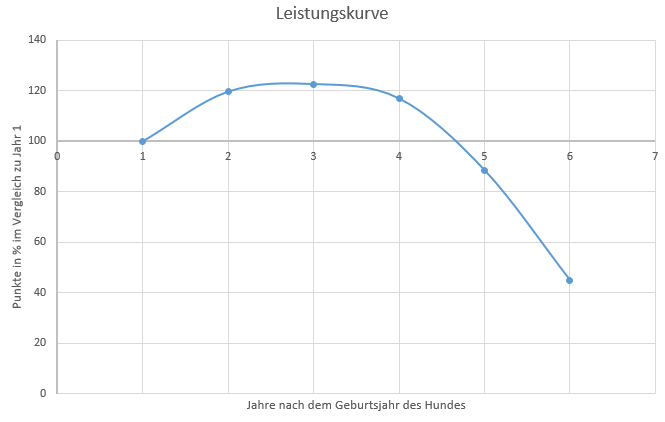
\includegraphics[width=1\linewidth]{leistungskurve}
			\caption{Leistungskurve über die durschnittliche Entwicklung der Hunde}
			\label{fig:leistungskurve}
		\end{figure}
		Mit diesen prozentualen Veränderungen haben wir mehrere Zukunftstabellen erstellt, abhängig davon, in welchem Jahr der Hund, den wir betrachten gelaufen ist. Wir haben für jedes Rennergebnis eine Prognose für alle folgenden Jahre erstellt, in denen der Hund noch aktiv ist und diese anschließend in der Tabelle \texttt{zukunft\_sauber} gemittelt. Auf diese Tabelle greifen wir mit unserer Webanwendung zu, um Vorhersagen über die Rennen unserer zufällig gewählten Hunde zu treffen.\\
		\\
		In postgres würde eine Anfrage für ein zufälliges Rennen im Jahr 2016 folgendermaßen aussehen:\\
		\\
		\texttt{
			SELECT zs\_name, zs\_score, zs\_year\\
			\hspace*{2mm}	FROM zukunft\_sauber\\
			\hspace*{2mm}	WHERE zs\_year = 2016 AND zs\_name IN (\\
			\hspace*{4mm}	SELECT name \\
			\hspace*{6mm}	FROM dog \\
			\hspace*{6mm}	WHERE year\_of\_birth > 2008 \\
			\hspace*{6mm}	ORDER BY random() LIMIT 6)\\
			\hspace*{2mm}	ORDER BY zs\_score DESC;\\
			}
			\\
		Die Einschränkung, dass die Hunde nach 2008 geboren sein müssen, sorgt dafür, dass wir nur zufällige Hunde wählen, die bei dem ersten imaginären Rennen noch mitlaufen können und nicht vor Beginn der Prognose schon ausgeschieden sind.\\
		\\
		Da es keine Hunde hab, die in ihrem 7. Lebensjahr noch gelaufen wären, haben wir für diesen Zeitraum keine Vorhersagen und bekommen die Ausgabe \texttt{NULL} obwohl die Hunde noch renntauglich wären.

	\subsection{Erweiterung der Web-GUI um Data-Mining-Aufgabe}
	Einmal die Web-GUI für generische SQL-Queries geschrieben, haben wir einfach eine neue JSP Datei erstellt, die speziell auf die Data Mining anfrage gemünzt wurd. Hier nun Eingabefelder für die 4 Hunde und Auswahlmöglichkeit des prognostizierten Jahres. Der Zugriff auf die Scoring Table für jeden Hund erfogte dann auf gleiche Art und Weise, wie die normalen Queries.
	
	
\end{document}